\documentclass[12pt]{article}

\usepackage{graphicx,amsmath,amssymb,multirow,rotate,color,subfigure}
\usepackage{float}

\setlength{\topmargin}{-.5in}
\setlength{\textheight}{9in}
\setlength{\oddsidemargin}{0.25in}
\setlength{\textwidth}{5.8in}

\begin{document}
\title{Usage and description of the code for steepest descent ballistic deposition of aggregates of spheres}
\author{Nikola Topic}
\maketitle
\tableofcontents
\section{Usage of the code}
The code generates packings of complex shaped particles by simulating the deposition process onto a horizontal plane set at $z=0$. The complex particles are composed of spheres of various radii and positions. The particles are dropped one by one, each particle follows the trajectory of the steepest descent of the center of mass until it reaches the stable position where it cannot descend anymore. In this position the particle is fixed and cannot be displaced by the following particles. The complete description of the model is given in "paper.pdf".
\subsection{Black box usage of the code}
The code uses the GNU Scientific Library for random number generation so it necessary to install it. When this library is available, compile the code by running \texttt{make} in the same folder as the code. A simple example can now be run with \texttt{./deposit 0.01 84328 3 1 1000 1 tmp}. The output should look like this:

\begin{verbatim}
user@msspc08:~/code_description$ ./deposit 0.01 84328 3 1 1000 1 tmp 
phi   0.01
Spiky particles
i   0
i   100
i   200
i   300
i   400
i   500
i   600
i   700
i   800
i   900
\end{verbatim}

The periodic boundary conditions are observed in horizontal $x$ and $y$ directions and particles are dropped over the periodic cell such that particles center of mass is uniformly distributed. The particles are randomly oriented before dropping.

After the run has finished, in folder "positions" a file named "positionstmp" is created that contains positions of the centers of spheres making up the complex particles. First three columns are $x$, $y$ and $z$ coordinates of the constituent spheres, while fourth contains the radii.  The filename "positionstmp" is obtained by adding the string that is the last parameter given to the function (in the example above it is "tmp") to the string "positions". Two additional files are also created. One in the folder "details" named "statetmp". To this file is written the number of particles sedimented and the number of intersection detected (it must be zero). Another file, named "cmstmp", is generated in the folder "cms". It contains the filling height of the sediment calculated as twice the height of the center of mass of the whole packing. The content to the files "statetmp" and "cmstmp" is append at the end of each simulation, while the file "positionstmp" is overwritten (unless the filename has been changed).

The particles that are deposited are "spiky" particles, identical to the one in Fig. 8(a) top. It is possible to chose from three particle shapes, mono-disperse spheres of radius 30 (fourth parameter =0), "spiky" particles (fourth parameter =1, as in the example above) and cube shaped particles (fourth parameter =2, figure 8(b) of the paper). For the spiky and cube shaped particles the particle sizes can be tuned by the third parameter, say denoted by n. In the example above $n=3$. For spiky particles n determines the number of spheres along an axis. Number of spheres along any of the axes is $2n-1$.  For the spiky particle in Fig. 8(a) $n=3$, which results in $5$ spheres along any of the axes. For the cube shaped particles, $n$ is the number of spheres along the side of the cube, equal to $5$ in Fig. 8(a) bottom. 

The number of dropped particles is determined by the fifth number (1000 in the example above). The sixth input parameter (equal to 1 in the above example) determines whether the cluster should be re-dropped in the (rare) case that special situations occur. Value of 1 means that cluster should be re-dropped. Changing the value between 1 and 0 helps in checking whether re-dropping has any influence on the packing.

First input parameter is the value $\Delta\varphi$ (see paper). The second input parameter is the seed for the random number generator. For an overview of parameter meanings see Fig. \ref{parameters}.

\begin{figure}
\includegraphics*[width=\columnwidth]{parameters.eps}
\caption{Input parameters.}
\label{parameters}
\end{figure}

%Changing the input file
Apart from the command line input parameters, the simulation can be controlled by the file "input". The 6 lines ("nx: 25" to "dz: 120") determine the size of the simulation volume. The extension of the periodic cell in $x$ direction is $nx*dx$ and in $y$ direction $ny*dy$. The largest height of the sediment that can be simulated is $nz*dz$. The quantity $dx$, $dy$ and $dz$ are sizes of cells into which the simulation volume is partitioned. Values of $dx$ etc. only affect the speed of the simulation, but not the result. The names of the output files can be changed in the last three line of the "input" file.

\subsection{Addition of a new particle shapes}

Arbitrary cluster shapes can be sedimented. To add a new particle shape it is necessary to add a function that generates this particle. This can be done by modifying an existing function, such as init\_sphere() in file "cluster.cpp". Make a copy of this function in the same file. Rename the function appropriately, and add it to the list of public functions of the class "clustertype" in file "cluster.h".

To add spheres to the cluster, in the newly created function fill vectors "r" and "R" with positions and radii of the spheres, respectively. Those spheres make-up the cluster to be sedimented. The cluster should be generated at large enough height such that it does not get into contact with the growing sediment. All clusters can have the same position and orientation, since they are randomly shifted horizontally over the periodic cell and randomly oriented before being sedimented in function main() in file deposit.cpp.  

%Center of mass determination
For non-overlapping spheres the center of mass of the cluster can be determined automatically with function cmass(). For cluster composed of overlapping spheres it is necessary to assign this value to the variable "cm".
%Note Rmax! 
If the radius of the largest sphere inside of the cluster exceeds the value "Rmax" in the file "common.cpp", then this largest radius  (plus a small value on the order of e.g. 10\% of the particle radius) should be assigned to Rmax.

To sediment this newly added cluster it is now necessary to generate clusters in the main() function. In deposit.cpp replace the line 33 with the following lines:

\begin{verbatim}
if(particle==3) ds("My new cluster");
if(particle!=0&&particle!=1&&particle!=2&&particle!=3) 
{
	ds("Not known particle shape");
	exit(1);
}
\end{verbatim}
This code will display the name of the new particle if it is chosen, and also the simulation will stop is non of the chosen particles is from the set ${1,2,3}$, with particle 3 newly added. It is also necessary to add after the line 43 (of the original unmodified "deposit.cpp") the line:
\begin{verbatim}
if(particle==3)	cp.init_my_new_cluster(nspheres);
\end{verbatim}
where "init\_my\_new\_cluster" should be the name of the new function created in "cluster.cpp". This initializes the particle. Before usage of the code it should be compiled by running "make". Now the new cluster can be sedimented by setting the fourth input parameter equal to 3, when running the code from the command line.

%Note about small polydispersity
When creating the cluster it is needed for the stability of the algorithm to add small polydispersity to spheres making up the cluster. If clusters are composed of just one sphere than they can have exactly the same radius - the code will work correctly.

If the radii of constituent spheres are around 30, then the default values $dx=120$, $dy=120$ and $dz=120$ in the "input" file are acceptable concerning the speed of the simulation.

\subsection{Changing the source of particles}
In the code the particles are dropped uniformly over the base of the periodic cell. The source of particles can be modified in the function main() in file "deposit.cpp". The assignment of initial particle positions and orientations before dropping is performed between lines 45 and 52 (of the unmodified code). 

In lines 41-43 the cluster (variable cp) is generated with its center of mass at position $(x=0,y=0,z=h0)$, where $h0$ is an initial (very large) height. In lines 45 to 52 (of the unmodified code) the cluster is translated horizontally to a random position over the periodic cell and rotated randomly. The positions to which the clusters are translated can be changed in line 45. The cluster will be translated by the vector $(ddx,ddy,0)$.

\subsection{Addition of fixed boundaries: ground, walls etc.}
The fixed boundaries composed of spherical particles can be added to the simulation. The particles making up the boundaries can be spread arbitrarily throughout the simulation volume. They should be added before the first moving particle is dropped. 

A single fixed sphere, set at $(1,1,1)$ with the default radius 30, is added by adding at line 59 in the file deposit.cpp the following code:
\begin{verbatim}
clustertype cp;
cp.init_sphere();
cp.r[0].x()=1;cp.r[0].y()=1;cp.r[0].z()=1;
unload(cp,su);
\end{verbatim}  
The cluster is composed of only one sphere and this sphere is positioned by directly modifying the cp.r vector containing the position of the sphere. Sphere is then added to the fixed particles with the line \texttt{unload(cp,su);}. By repeating this procedure more spheres can be added. Again, if the radius of any of the fixed spheres exceeds the value \texttt{Rmax} in file "common.cpp", the value of \texttt{Rmax} should be increased to be larger than the largest radius.

%Usage of walls
The default simulation sediments particles onto a flat horizontal plane, with particles becoming fixed on the first contact with the ground. If the ground is covered with fixed spheres than the cluster can roll on the ground. Likewise, fixed particles can be of use to simulate e.g. walls of a container.

\section{Code description}
In this section the code will be described completely, file by file and function by function. The files are grouped into three section, and each subsection corresponds to a single .cpp and a single .h file with the same name.
\subsection{main() function, input/output and global variables}
\subsubsection{deposit.cpp}
The file "deposit.cpp" contains the main() function. In this function the simulation is initialized, clusters are generated, sedimented and output files are created.

In line 11 the random number generator for the Gnu Scientific Library is initialized (apart from random number seed). In the following line, line 12, the file "input" will be read and the values are assigned to global variables. Those two functions are defined in "functions.cpp".

In lines 16 to 19 the value of $\Delta\varphi$ is read from the command line and assigned to global variable \texttt{phi}. This overwrites the value given in the file "input". The cosines and sines are calculated immediately afterwards, and assigned to global variable \texttt{rotinfphi}. The global variable is used whenever a rotation by $\Delta\varphi$ is performed. This variable if of type "rotinftype" and which is defined in file "rotinf.h". In lines 21 and 22 seed for the random number generator is read, and its value is passed to GSL function "gsl\_rng\_set". In lines 24 to 28 the other parameters are read from the command line.  

In lines 38 to 55 the clusters are generated and and added to vector \texttt{co} which contains clusters to  be sedimented. The clusters are generated inside of the loop since each cluster differs by small amounts in positions of spheres in it. After being randomly placed over the base of the periodic cell they are randomly rotated around their center of mass with function "randrot" which is a member of class "clustertype".

In lines 57 to 58 the object "su" is initialized. This object stores all the information about fixed particle, i.e. about the surroundings of the cluster. Its corresponding type is defined in "surround.h" and "surround.cpp" and discussed in more details in the section "surround". 

In lines 60 to 92 the clusters from vector "co" are sedimented using the function "settle" which settles the cluster considering the surroundings. This is done by the call \texttt{c.settle(su)}, where "c" is the cluster to be sedimented. In some situations the cluster needs to be re-dropped, for example if cluster after collapse has two contacts with one fixed particles, or if the cluster is progressing very slowly. Once the sedimentation is complete the cluster added to surroundings with a command \texttt{unload(c,su)}, defined in "function.cpp".  

Once all clusters are sedimented the details about the simulation are outputted.
\subsubsection{functions}
The two files "functions.h" and "functions.cpp" contain functions that are useful in "main" function such as, random number initialization, input output of data, checking for overlaps within the sediment etc..

The function "initrand" initializes the state of the GNU Scientific Library random number generator. The seed is provided in the main function in "deposit.cpp". The function "load\_parameters" reads parameters from a file (by default file name "input" in the same folder as the code) containing simulation parameters. Those parameters assigned to corresponding global variables defined in "common.h" and "common.cpp". 

Function "cmass()" calculates the center of mass of the set of non-overlapping spheres given by the vector "r" containing the positions of spheres and vector "R" containing the radii. This function is useful in calculating the filling height of the sediment, since the filling height can be approximated as twice the height of the center of mass of the packing. 

Function "checkinters" checks whether there are any intersection inside of the sediment. It returns the total number of intersection. If the cluster contains overlapping spheres than it will also report that there are intersection. The function after this is also named "checkinters", however it takes as an input a single cluster and the object containing the sediment (surroundings). This function check whether there are any intersection between that single cluster and the fixed particles. It does not check for overlaps within the cluster or withing the sediment, only for overlaps between pairs of spheres where one is from the cluster and another one from the sediment. This function is useful for debugging purposes. 

The next function is "find\_cluster\_contacts". It finds the contacts that a cluster has with particles from the surroundings. Whether two spheres touch or not is driven by parameter "eps\_contact". If distance between particle surface is smaller than "eps\_contact" the particle are considered as touching. This function is of great importance since it is used to detect contacts when the cluster is in the collapsed state. 

Functions "unload" and "unloadsphere" are used to add the cluster into the fixed particles. More details discussion of those two function is given in section "Objects", subsection "surround". The rest of the functions in this file write out the details of the simulation. The function \texttt{output(surroundtype\& su,string fname)} outputs the positions of and radii of fixed spheres. The clusters are cut by the periodic boundary conditions. Similar function \texttt{void output(vector<clustertype>\& cd,string fname)} outputs into a single file position of spheres belonging to clusters in vector "cd". The clusters are not cut by the periodic boundary conditions. The function "writedetails" outputs to a file the number of clusters that were sedimented and the number of intersections. Finally, "write2cm" writes the filling height of the sediment to a file. 
\subsubsection{common}
Files "common.h" and "common.cpp" are intended to contain variables and short functions that are used throughout the code. "common.h" is included in most of the other files. 

The functions of note in "common.h" are "ranf", which returns uniformly distributed number in the interval $[0,1)$ and "ranfs" which returns uniform random numbers in the interval $[-1,1)$. In file "common.cpp" the function "rand\_orientation" returns vectors uniformly distributed on a unit sphere.

The meaning of variables in file "common.cpp" between the lines 7 and 20 is discussed in section "Objects", subsection "surround", and in section "file "input"". 

\subsubsection{short\_cout.h}
The file contains definition of a function "ds()" which can display up to 10 values, either text or numbers, or variables of type "vtype" (see section "SimpleVector.h") onto the screen. For example \texttt{ds("Number:",1,3);} will display "Number: 1 3".
\subsection{Objects}
In this section the two most important types will be discussed: "clustertype" and "surroundtype". With them the clusters are manipulated in the simulation. 
\subsubsection{surround}
The class "surroundtype" contains all the fixed particles. Once the cluster is sedimented it is added to the surroundings such that it provides a surface for future clusters to roll on.
\begin{figure}[!htbh]
\includegraphics*[width=\columnwidth]{grid.eps}
\caption{Organization of the simulation lattices and names of variables.}
\label{lattice}
\end{figure}
Class "surroundtype" is defined in the file "surround.h". The data members "r" and "R" contain the positions and radii of the fixed particles. The variable "box" corresponds to a 3 dimensional lattice where each cell contains the indexes of particles that belong to it. A two dimensional representation of variable "box" and corresponding variables is shown in Fig. \ref{lattice}. In the simulation the lattice extends also in the horizontal y direction, with analogously named variables for $y$ direction. In the simulation the variable "izmax" is a two dimensional lattice, corresponding to horizontal x and y directions, that stores the $z$ index of the highest occupied cell of the three dimensional lattice. For a two dimensional analog of a three dimensional grids used in the simulation in Fig. \ref{lattice}, izmax variable is one dimensional and izmax[0] is 0 and izmax[4] is 2. The values \texttt{x0,y0} can be set to 0, however the value of \texttt{z0} should be negative, since when the cluster is rolling near the ground some checks below the ground plane $z=0$, and this will cause an error if there are no cells, even empty ones below the ground plane.

%grid init discuss
Function \texttt{init\_grid} initializes the box and izmax variables such that they are ready to receive particles information. The variables nx, ny and nz are global variables defined in common.cpp and their values are assigned either in functions.cpp, in function \texttt{load\_parameters}, where their values are read from file "input". 
%unload mention
The function \texttt{unload} that adds a cluster into the surroundtype variable is defined in functions.cpp. In this function (and with the help of function \texttt{unloadpshere}), cluster spheres positions and radii are appended to corresponding vectors in the object of type surroundtype, their indexes added to the variable \texttt{box} and variable \texttt{izmax} is updated.

\subsubsection{cluster}
The classes and their functions defined in "cluster.h" and "cluster.cpp" are central to the simulation, since they are used to represent and sediment the cluster. Operation in those two files focus more on the operation with objects, finding new events moving the cluster etc., while pure "low level" numerical calculations with vectors are shifted mostly to files "numerics.h" and "numerics.cpp".  

The purpose of the class clusterbase is to store the information about the cluster that is useful for a rigid body composed of spheres, but without details such as positions of the sphere centers. The classes that describe for example a possible future position of the cluster, or the complete cluster representation are derived from this class. The variable \texttt{contacts} is the number of contacts that a cluster currently has, while variable stable has value true if the cluster is stable otherwise false. The pair \texttt{d1,p1} contain the index of the cluster sphere and index of the fixed sphere, respectively, that are in contact. If they are not in contact then they have value $-1$ or another appropriately chosen negative value. \texttt{d2,p2} and \texttt{d3,p3} have analogous meanings for the second and third contact. The variables \texttt{td,tp} are help variables used when a contact needs a special attention. Variable \texttt{f} is true if the cluster lost one contact in the previous step by situation in Fig. 6a of the paper, otherwise it is false. Variable \texttt{cm} stores the value of the center of mass of the cluster. Which cluster has higher center of mass can be determined with operators \texttt{<} and \texttt{>}.

The class \texttt{fallattempt} is used to represent the cluster in test positions when the cluster is falling. No additional variables compared to \texttt{clusterbase} are needed.

The class \texttt{rotattempt} represents the cluster in text positions when the cluster is rotating. It contains a new variable \texttt{rotinf}, of type \texttt{rotinftype} defined in "rotinftype.h" and "rotinftype.cpp". The variable contains the axis of rotation and cosines and sines of the angle of rotation by which the cluster needs to be rotated from the current position to reach the future test position.

The class \texttt{gradrotattempt} contains additional information compared to \texttt{rotattempt}, namely the variable \texttt{gz} into which is stored how steeply does the center of mass descends in the test position. The value stored into this variable is the scalar product of axis $\vec e_z$ pointing upwards and the unit vector tangential to the trajectory of the steepest descent pointing in the direction of the movement of the center of mass. This type is useful when there are many possible descent trajectories for the same position of the cluster and the steepest one is searched. 

Finally, the class \texttt{clustertype} is the full implementation of the cluster object. It contains functions for handling the cluster. The variables \texttt{r} and \texttt{R} are positions and radii of the spheres making up the cluster. The positions of the spheres are updated whenever the cluster moves. The function \texttt{cmass} determines the centers of mass of the cluster. It can be used only when the cluster spheres are non-overlapping, since otherwise it will likely give an incorrect value. The function \texttt{erase} empties the vectors \texttt{r} and \texttt{R}. The functions are now discussed in the order as they appear in "cluster.h". 

The member function \texttt{init\_sphere()} initializes object such that it contains one sphere of radius 30, placed at position $(0,0,h0)$, where $h0$ is a very large height, defined in "common.cpp". The functions \texttt{init\_axes\_lines\_mshuffle} and \texttt{init\_cube\_mshuffle} initialize the clusters from Fig. 8a top and bottom, respectively (although with adjustable size of the cluster). The variable \texttt{nsph\_per\_side} determines the size of the cluster. The variable \texttt{eps\_sh} determines the amount by which the sphere positions are randomly shifted in random direction from their ideal positions. If such random shift are not added the cluster may get into a motion where it is moving very little between events, but still descends, for a very large number of events.

Function \texttt{settle} is the most important function of the whole code. Is calculates the position of the cluster after if performs the movement on the previously dropped particles. The final position of an object say \texttt{c} of the type \texttt{clustertype} sedimented onto fixed particles stored in the variable \texttt{su} of the type \texttt{surroundtype} can be calculated by calling \texttt{c.settle(su)}. The while loop of the function loops until the cluster reaches a stable position. The \texttt{switch} choses between three functions to be executed depending on the number of contact the cluster has. Each of three functions \texttt{fall,rotate1,rotate2} move the cluster by one event. After the cluster moves by one event, it is checked whether its center of mass has moved by more than \texttt{eps\_collapse} distance. If not, it may be that the cluster is close to a collapsed position. The clusters contacts are then recalculated using the function \texttt{find\_cluster\_contacts}, which calculates cluster contacts by considering a contact closed if the distance between a fixed particle and a cluster particle is below \texttt{eps\_contact}. If such situation is detected by chance and cluster is not in collapsed situation, this is not a problem since the steepest descent trajectory is chosen, in agreement with the rules of the motion. It then checked whether one cluster sphere contacts two fixed particles, and the truth value is assigned to \texttt{duplicate\_exists}. If there are such contacts the dynamics is considered undefined and \texttt{collapsed} variable receives value true, movement of the cluster is stopped and the decision whether to re-drop the cluster or freeze it in its current position is made in the \texttt{main} function. Such situations are rare, appear typically on the order of few thousand particles. If there are no such contacts, all closed contacts are considered and the new steepest descent trajectory is chosen. Additional check is performed, whether cluster is making progress. If cluster does not move by more than $60$, or about one constituent sphere diameter in last one million events the decision is made in the \texttt{main} function whether cluster is redropped or its position is considered final. 

The function \texttt{periodic} moves the cluster to the periodic cell when the clusters center of mass exits the cell as the cluster moves. The whole cluster is translated horizontally by the same vector with the function \texttt{movecluster}. The variables \texttt{pxb,pyb} are the coordinates of the beginning of the periodic cell and \texttt{lx,ly} are the extensions of the periodic cell in horizontal directions. Those are global variables declared in "common.h" and "common.cpp" and their values are assigned in function \texttt{load\_parameters} in "functions.cpp". Function \texttt{randrot} randomly rotates the cluster. The random rotation is preformed by transforming the cluster to a randomly chosen coordinate system.

The following functions do everything with respect to propagating the cluster by one event. 

The function \texttt{fall} moves the cluster to the the first collision when the cluster is falling, and updates the state of the cluster such that is has one contact. Variable \texttt{atvec} contains the vector of possible future events. Possible future events are of the type \texttt{fallattempt}. This data type contains all the information about the cluster including its center of mass in the new position, but does not include the position of the cluster spheres. If this event is chosen the position of the spheres in the cluster can be obtained from the distance that center of mass traveled. Memory is saved by not storing the position of the constituent spheres in the possible future events, but only the essential information for the event. Function \texttt{bfall} finds possible future events where there is a collision of the cluster with the fixed spheres, and adds them to event vector, while \texttt{gfall} finds possible future collisions with the ground. Then the event which happens at highest hight (but in the future) is chosen, and the cluster is moved to this position using the \texttt{step0} function.

As mentioned above the function \texttt{bfall} deals with collisions with fixed spheres when the cluster is falling, and finds such candidate future events. The search for collisions is performed for each sphere in the cluster, and in the code this is the for loop for variable \texttt{k}. For candidate fixed sphere \texttt{j} it is check whether collision is possible using the function \texttt{pcontact0}. This function is defined in "numerics.h" and "numercis.cpp". If there is such collision the amount of translation distance the cluster sphere \texttt{k} moves in order to collide with the fixed sphere \texttt{j} is written to variable \texttt{dlt}. The collision is now considered as a possible future event and to the \texttt{att} of type \texttt{fallattempt} are assigned appropriate values for this collision. The cluster is unstable and has one contact. Finally, if the center of mass is lower than the current when this collision occurs, the event is added to the list of possible events. To find fixed particle candidates that have a high probability of being a collision partner, grid information in variable \texttt{su} of type \texttt{surroundtype} is used, namely the variable \texttt{box} that stores indexes of fixed particles. The indexes of boxes that contain candidate fixed spheres are between and including \texttt{ixl,ixr} and \texttt{iyl,iyr}, when adjusted according to periodic boundary conditions they are renamed as \texttt{i} and \texttt{n}, and for the $z$ index \texttt{m} between \texttt{izmax[i][n]} and 0. Lower bound for \text{m} is improves (or stay the same) when a collision is detected, since it is not necessary to search boxes whose \texttt{m} index is smaller than \texttt{floor((zfc-R[k]-Rmax-zo)/dz)))}, where \texttt{zfc} is the current highest height of the center of sphere \texttt{r[k]} in position where it contacts its corresponding collision partner. The purpose of the line \texttt{if(k!=td||j!=tp)} is to avoid recontact when the contact is lost in the previous step by rolling to horizontal (Fig. 4b of the paper). Further optimizations are possible, but not necessary, since even with current optimization this function takes a small fraction of time compared to function when the cluster is rotating.

The next function is \texttt{gfall} function which finds potential events when the cluster is colliding with the ground plane $z=0$. The cluster is considered considered stable when it hits the ground plane. Finally function \texttt{step0} assigns the information from the chosen event to the cluster, and moves it to that new position, with the help of function \texttt{translate}. One thing of importance in function \texttt{translate} is the correction of the position of cluster sphere which make a new contact, such that it is in contact with the fixed particle with higher precision (this moves the cluster sphere only by a small amount on the order of $10^{-9}$). \texttt{eps} is a global variable defined in "common.cpp".

The function \texttt{rotate1} moves the cluster to the next event when the cluster has one contact. Its  structure is analogous to the structure of the \texttt{fall} function, only that there are now more possibilities for future events. Those cases are discussed in the paper. In this function the case is treated when the center of mass \texttt{cm} is exactly on top fixed particle on which the rotation should be performed. If uncorrected it causes problems since the axis of rotation is undefined. To correct this situation the fixed particle is shifted in a random horizontal direction by a very small amount, and after the event is performed the fixed particle is returned to its original position. 

The function \texttt{steeperdphi} deals with the "frustrated" situations, described in the section 4.1 of the paper. In this function first it is checked whether the cluster really is in the frustrated situation, by checking whether cluster sphere is below the fixed sphere on which the rotation should be performed. If this is the case then the event where cluster is allowed to fall is added (depending on details) to the vector of possible events. In that event the cluster is rotated by angle $\Delta\phi$ (whose cosines and sinuses are stored in the global variable \texttt{rotinfphi}) around an axis (see paper) through the center of the fixed particle. As mentioned above, whether the cluster state after the rotation is a valid event needed to be checked before an event is added to the event list. First it is checked whether the clusters center of mass after the rotation, \texttt{cmc}, is still on the same side of the vertical plane containing the rotation axis. If it is not true it implies that the center of mass has swung past the lowest point, which is not possible since the height of the center of mass would have to increase. Finally, a check is made whether the cluster sphere is still below the fixed sphere, and if this is true the event is added to the vector of events. 

The function \texttt{brot1} finds potential collisions with fixed spheres while the cluster is rotating on one contact. The central function called by \texttt{brot1} is \texttt{pcontact1}, which implements the solution from the paper in section 3.2.2. The function \texttt{pcontact1} solves the system of equations (7)-(9) of the paper (see also Fig. 5 of the paper). It is defined in "numerics.h" and "numerics.cpp". The function \texttt{pcontact1} tests whether a collision is possible between a fixed sphere, with index \texttt{j} and cluster sphere with index \texttt{k}, and calculates the rotational information stored in variables \texttt{rotinf1} and \texttt{rotinf2} (two solutions for each collision), if collision is possible. It solves the. If collision is possible and event is a valid future event, the steepest descent trajectory on existing contacts is found using the \texttt{find\_steppest\_descent} function. The commands \texttt{rightside(cm-rp,cmc-rp,rotinf.n)} check whether the center of mass has swung past its lowest point, \texttt{g(rp,cmc,rcc,rp2)<0} checks whether cluster sphere "pushes" into the fixed particle as the cluster rotates in the direction of steepest descent. With \texttt{cmc.z()<cm.z()+epsz} it is checked whether the center of mass in the new position is lower than in the previous. \texttt{epsz} is a very small number defined in "common.cpp" which allows very small increase in height, which are necessary when for example mono-disperse packing of spheres has crystalline structure, causing valid events in which very small increase in height appears, caused by the finite precision of the number representation.  
%optimization

\begin{figure}[!htbh]
\begin{center}
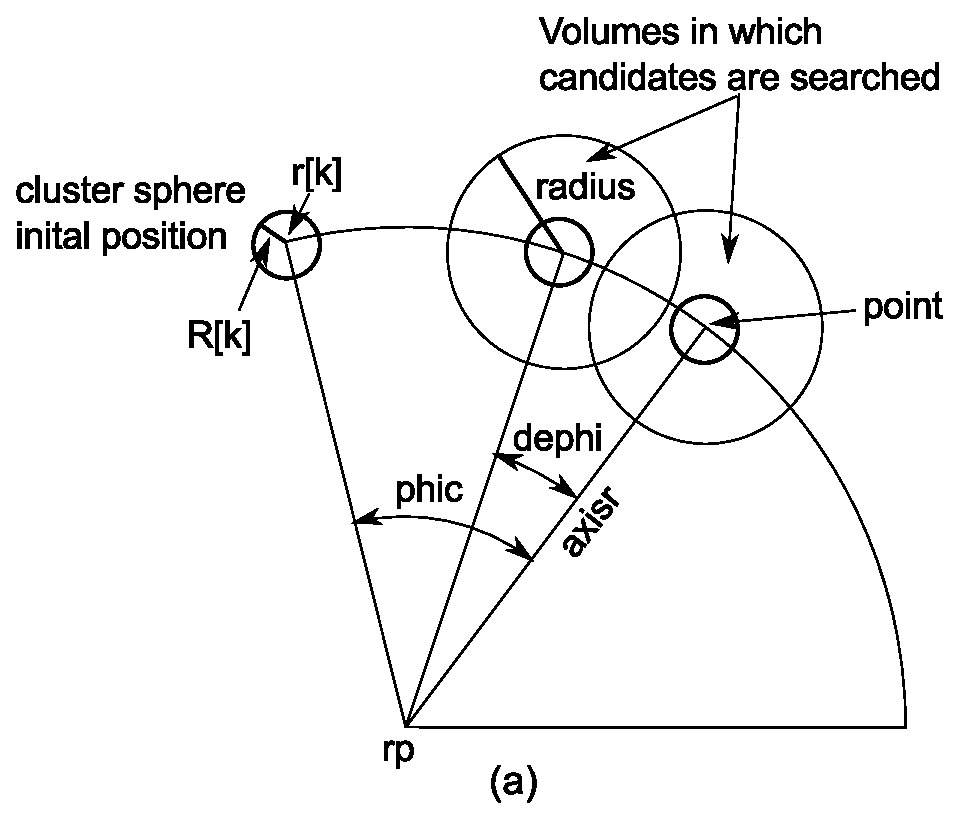
\includegraphics[width=0.54\textwidth]{drawing_optimization_final_a.eps}
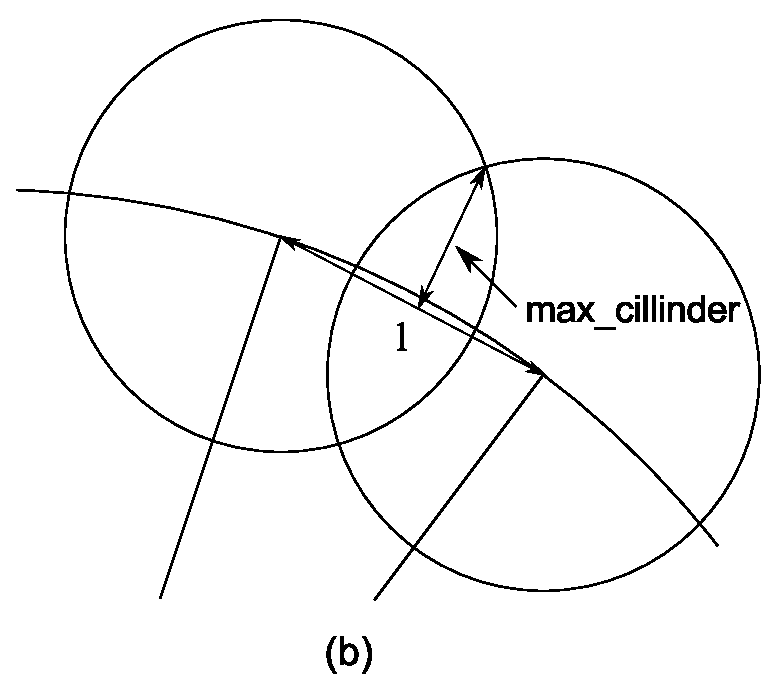
\includegraphics[width=0.44\textwidth]{drawing_optimization_final_b.eps}
\caption{Geometry of the search for candidates, with variables named same as in the code. For clarity the sketch is made in two dimensions. The generalization to three dimensions is straightforward.}
\label{optim}
\end{center}
\end{figure}


The rest of the function \texttt{brot1} is devoted to efficient search for candidate collision partners. To first contact of the cluster with fixed particles corresponds the minimal angle of rotation of the cluster, in the direction of steepest descent. For each sphere inside the cluster there are a number of angles (possibly zero), at which this sphere make a contact with spheres from the surroundings. The number of checks for contacts can be dramatically reduced by considering only fixed particles which are in the vicinity of circle that a sphere from the cluster makes while rotating around the axis, Fig. \ref{optim}a. To find candidates for contacts the sphere is rotated around the axis in discrete steps with angle of rotation \texttt{dephi} and in each step candidates are taken within the distance \texttt{radius} from the current position. The size of discrete steps must be such that the search neighborhoods in consecutive steps are overlapping enough so that none of the possible candidate particles are missed, Fig. \ref{optim}b.  The condition that no collision partner is missed is \texttt{max\_cylinder<=R[k]+Rmax}. Search of particles within the neighborhood of radius \texttt{radius} is performed with the help of the grid, \texttt{su.box}.

To find the first contact of the cluster with the surroundings, cluster is rotated as a rigid body by some fixed angles \texttt{dephi}. In each position \texttt{phic}, the candidates are searched within some neighborhood of each particle of the cluster as described in the previous paragraph. For each cluster test angle \texttt{dephi} candidates are searched and tested for collision. The search is stopped when \texttt{phic>phidet+dephi}.  The value of \texttt{dephi} was chosen such that particle at the highest distance from the axis has $l=2(R_{max}+R[k])$. When cluster sphere with the largest distance from the axis has $l<radius$ then $dephi=60^{\circ}$, with $l$ recalculated accordingly. 

The function \texttt{hrot} adds event for the case in Fig. 4b of the paper. The important function is \texttt{tohorizontal} which calculates the amount of rotation, stored in \texttt{rotinf}, needed for the cluster spheres \texttt{d1} to have the same height as fixed sphere at \texttt{rp}.

The function \texttt{grot1} adds event where the cluster is rotated such that it touches the ground. To find the contact of one cluster sphere with the ground the function \texttt{toground1} (defined in "numerics.h" and "numerics.cpp") is used. Finally, an event is added in function \texttt{bottomrot1} where cluster hangs on one contact with the center of mass below the fixed particle. In function \texttt{step1} the cluster's state is updated when cluster has one contact.

The function \texttt{rotate2} has analogous purpose and structure to function \texttt{rotate1} except that cluster is rotating on two contacts. In this function it is necessary to repair the situation which occurs when the center of mass of the cluster is exactly above the line connecting centers of fixed particles, and therefore the direction of rotation is undefined. This situation is repaired with the same approach as the similar situation in \texttt{rotate1}, namely one of the fixed particles is moved by a very small amount, and then moved to its original place, once the cluster is propagated.

The function \texttt{steeperdphi2} is analogous \texttt{steeperdphi}, except that cluster has two contacts. First it is checked whether there is steeper descent i.e. whether cluster can move with less contacts (statement \texttt{if(att.contacts<contacts)}). If so, the cluster is rotated by a small angle and a new set of contacts is calculated which is consistent with steepest descent path. It is necessary to first rotate the cluster before it can move on a new steeper trajectory. In Fig. 7a of the paper is an example for rotation on one contact, where cluster first needs to rotate by a small angle before it can move on the steeper trajectory.

Functions \texttt{brot2,bottomrot2,grot2,hrot2} are very similar to their analogous functions \texttt{brot1,bottomrot1,grot1,hrot}, respectively, with only difference being that they are adapted for the cluster rotation on two contacts instead of one.

The function \texttt{disconnect} adds events for the situation from Fig. 6a section 3.3.3 of the paper. The function that performs the most important computation is \texttt{pdisconnect}, which solves equation (25) of the paper and finds the amount of rotation of the cluster, stored in rotinf1 and rotinf2 (two solutions are possible), for the Eq. (25) to be satisfied. The function \texttt{pdisconnect} is defined in "numerics.h" and "numerics.cpp". The function \texttt{disconnect} is organized in the following way. First it is checked whether contact 2 is closing when the rotation is solely on contact 1, i.e. $\vec{t}_{1,2}\left(\vec{r}^{\,a}_2-\vec{r}^{\,s}_2\right)<0$, which in the code is done in line \texttt{bool push12=g(rp1,cm,rd2,rp2)<0;}. The function \texttt{g} is discussed in full in section devoted to "numerics.cpp". If the contact is closing then with \texttt{pdisconnect} two solutions are found where $\vec{t}_{1,2}\left(\vec{r}^{\,a}_2-\vec{r}^{\,s}_2\right)=0$. Then each solution is considered. First it is checked for the first solution whether condition (31) of the paper is satisfied, with the help of function \texttt{positivecircle}\footnote{In the paper condition is written for contact 1, but analogous relation can be written for contact 2 while rotating on contact 1}. If the condition is not satisfied an event is added where contact 2 is considered open and cluster allowed to freely rotate on the first contact. If condition (31) is satisfied, then cluster is rotated by a small angle and then if contact 2 is still opening the event is added to the event vector. The same procedure is done for the other solution, and then for the loss of contact 1 if \texttt{push21=g(rp2,cm,rd1,rp1)<0;} has value \texttt{true}.
\begin{figure}[!htbh]
\begin{center}
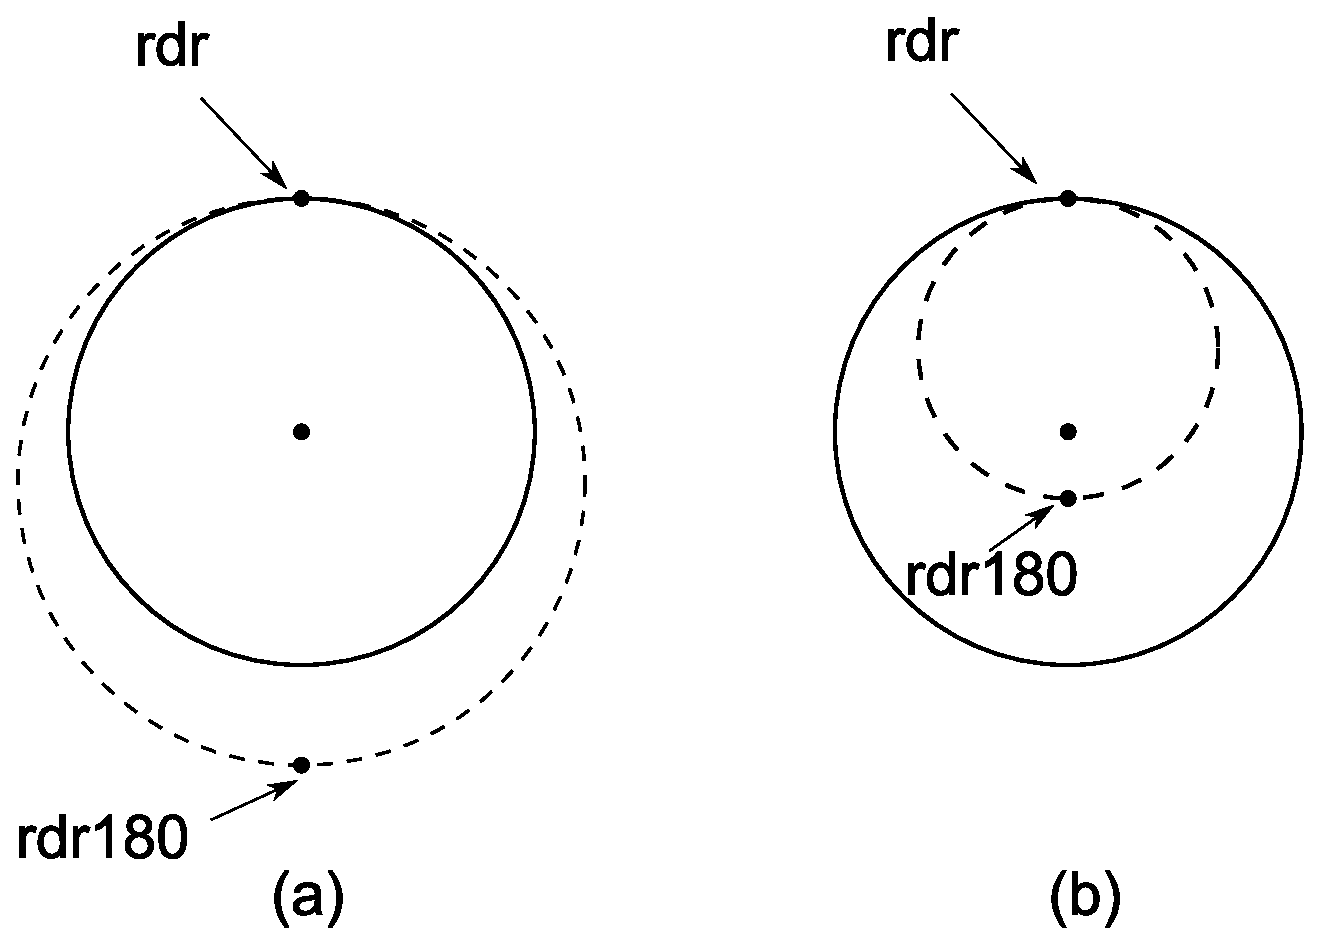
\includegraphics[width=0.54\textwidth]{positive_circle.eps}
\caption{Schematic drawing of the test whether condition (31) of the paper is satisfied or not, performed in function \texttt{positivecircle}. The variables have same names as in the code.}
\label{positive}
\end{center}
\end{figure}

Function \texttt{positivecircle} determines whether condition (31) is satisfied or not. Since $\vec{t}_{1,2}\left(\vec{r}^{\,a}_2-\vec{r}^{\,s}_2\right)=0$ is automatically satisfied it is only checked that $\frac{d^2}{d\varphi^2}\left|\vec{\varrho}^{\,a}_2-\vec{r}^{\,s}_2\right| < 0$, Fig. \ref{positive}. Starting from the position where $\vec{t}_{1,2}\left(\vec{r}^{\,a}_2-\vec{r}^{\,s}_2\right)=0$ (position rdr in the code), the cluster sphere is rotated 180 degrees (position rdr180 in the code) as if the whole cluster is rotated only on contact 1, with motion according to rule in Fig2b of the paper. If the cluster sphere at contact 2 is now further away from the fixed sphere at contact 2 then before rotation by 180 degrees, then $\frac{d^2}{d\varphi^2}\left|\vec{\varrho}^{\,a}_2-\vec{r}^{\,s}_2\right| > 0$, Fig. \ref{positive}a, otherwise $\frac{d^2}{d\varphi^2}\left|\vec{\varrho}^{\,a}_2-\vec{r}^{\,s}_2\right| < 0$, Fig. \ref{positive}b at position where $\vec{t}_{1,2}\left(\vec{r}^{\,a}_2-\vec{r}^{\,s}_2\right)=0$ is valid (\texttt{rdr} in the code). 

The function \texttt{step2} updates the state of the cluster according to chosen event when cluster has two contacts. The function \texttt{find\_steppest\_descent} finds the set of contacts (may be empty, which implies falling) on which cluster to rotate such that the center of mass descends the steepest. 

\subsection{Numerics}
In this section functions that focus no purely numerical calculations are discussed. 
\subsubsection{numerics}
Code in "numerics.h" and "numerics.cpp" contains numerical routines that are used in "cluster.cpp". Routines deal exclusively with scalar and vector inputs, and implement solutions of problems discussed in the paper.

Function \texttt{pcontact0} finds translation length such that one sphere translating vertically collides with a fixed sphere (section 3.1 of the paper). Function \texttt{pcontact} finds a solution for situation in Fig 5 of the paper. Function \texttt{circle\_intersect} finds intersections between two circles one at (0,0) another at (d,0). The function \texttt{pcontact1} adapts the function \texttt{pcontact} for collision of one sphere with fixed, while cluster is rolling on one contact. Function \texttt{tohorizontal} implements the solution from section 3.2.3 of the paper, function \texttt{tobelow1} from section 3.2.4, and \texttt{toground1} from 3.2.4. Function \texttt{g} calculates $\vec{t}_{1,2}\left(\vec{r}^{\,a}_2-\vec{r}^{\,s}_2\right)$. While function \texttt{grad} calculates the unit vector in which the center of mass moves when cluster is rotating on one particle. 

Functions \texttt{pcontact2,pdisconnect,tohorizontal2,tobelow2,toground2} implement solutions from sections 3.3.2-3.3.6 of the paper, respectively. Function \texttt{g2} and \texttt{grad2} are analogs of \texttt{g} and \texttt{grad}, but for rotation on two contacts.

The function \texttt{rightside} is highly used. It determines whether the center of mass is on the same side of a vertical plane containing rotation axis, before and after the rotation. Function \texttt{planecontact} finds a contact of a point with a horizontal plane, while rotating around axis \texttt{n}.

The function \texttt{findindex} finds upper and lower bounds for indexes of grid boxes in the surroundings of a sphere. The size of the surrounds includes only boxes that may contain spheres that touch the sphere being considered. The function \texttt{distance\_from\_axis} finds distance of point \texttt{rc} from the axis when motion is according to rule from Fig. 2b of the paper. \texttt{findpoints} finds points (Fig. \ref{optim}a of this document) that correspond to positions of point \texttt{r[k]} where the neighborhood is searched for collision partners. The function \texttt{rotpoint} rotates a point around axis defined by \texttt{rp} and \texttt{cm} (Fig. 2b of the paper). Functions \texttt{distance\_from\_axis2,findpoints2,rotpoint2} are analogous, with rotation being on two contacts.

\subsubsection{mod, matrix, rotinf, SimpleVector.h}
Those files contain object definitions for modular operations, matrix operations (subset of basic operations) and storing the information about rotation (angles and rotation axis) and for implementation of vector class (original developer is Thomas Schawger, here it is somewhat extended), respectively.

\subsection{file "input"}
File "input" controls the parameters of the simulation that are not controlled from the command line.
\end{document}

